%----------
%   WARNING
%----------

% This Guide contains Library recommendations based mainly on APA and IEEE styles, but you must always follow the guidelines of your TFG Tutor and the TFG regulations for your degree.

% THIS TEMPLATE IS BASED ON THE IEEE STYLE 


%----------
% DOCUMENT SETTINGS
%----------

\documentclass[12pt]{report} % font: 12pt

% margins: 2.5 cm top and bottom; 3 cm left and right
\usepackage[
a4paper,
vmargin=2.5cm,
hmargin=3cm
]{geometry}

% Paragraph Spacing and Line Spacing: Narrow (6 pt / 1.15 spacing) or Moderate (6 pt / 1.5 spacing)
\renewcommand{\baselinestretch}{1.15}
\parskip=6pt

% Color settings for cover and code listings 
\usepackage[table]{xcolor}
\definecolor{azulUC3M}{RGB}{0,0,102}
\definecolor{gray97}{gray}{.97}
\definecolor{gray75}{gray}{.75}
\definecolor{gray45}{gray}{.45}

% PDF/A -- Important for its inclusion in e-Archive. PDF/A is the optimal format for preservation and for the generation of metadata: http://uc3m.libguides.com/ld.php?content_id=31389625. 

% In the template we include the file OUTPUT.XMPDATA. You can download that file and include the metadata that will be incorporated into the PDF file when you compile the memoria.tex file. Then upload it back to your project.  
\usepackage[a-1b]{pdfx}

% LINKS
\usepackage{hyperref}
\hypersetup{colorlinks=true,
	linkcolor=black, % links to parts of the document (e.g. index) in black
	urlcolor=blue} % links to resources outside the document in blue

% MATH EXPRESSIONS
\usepackage{amsmath,amssymb,amsfonts,amsthm}

% Character encoding
\usepackage{txfonts} 
\usepackage[T1]{fontenc}
\usepackage[utf8]{inputenc}

% English settings
\usepackage[english]{babel} 
\usepackage[babel, english=american]{csquotes}
\AtBeginEnvironment{quote}{\small}

% Footer settings
\usepackage{fancyhdr}
\pagestyle{fancy}
\fancyhf{}
\renewcommand{\headrulewidth}{0pt}
\rfoot{\thepage}
\fancypagestyle{plain}{\pagestyle{fancy}}

% DESIGN OF THE TITLES of the parts of the work (chapters and epigraphs or sub-chapters)
\usepackage{titlesec}
\usepackage{titletoc}
\titleformat{\chapter}[block]
{\large\bfseries\filcenter}
{\thechapter.}
{5pt}
{\MakeUppercase}
{}
\titlespacing{\chapter}{0pt}{0pt}{*3}
\titlecontents{chapter}
[0pt]                                               
{}
{\contentsmargin{0pt}\thecontentslabel.\enspace\uppercase}
{\contentsmargin{0pt}\uppercase}                        
{\titlerule*[.7pc]{.}\contentspage}                 

\titleformat{\section}
{\bfseries}
{\thesection.}
{5pt}
{}
\titlecontents{section}
[5pt]                                               
{}
{\contentsmargin{0pt}\thecontentslabel.\enspace}
{\contentsmargin{0pt}}
{\titlerule*[.7pc]{.}\contentspage}

\titleformat{\subsection}
{\normalsize\bfseries}
{\thesubsection.}
{5pt}
{}
\titlecontents{subsection}
[10pt]                                               
{}
{\contentsmargin{0pt}                          
	\thecontentslabel.\enspace}
{\contentsmargin{0pt}}                        
{\titlerule*[.7pc]{.}\contentspage}  


% Tables and figures settings
\usepackage{multirow} % combine cells 
\usepackage{caption} % customize the title of tables and figures
\usepackage{floatrow} % we use this package and its \ ttabbox and \ ffigbox macros to align the table and figure names according to the defined style.
\usepackage{array} % with this package we can define in the following line a new type of column for tables: custom width and centered content
\newcolumntype{P}[1]{>{\centering\arraybackslash}p{#1}}
\DeclareCaptionFormat{upper}{#1#2\uppercase{#3}\par}
\usepackage{graphicx}

% Table layout for engineering
\captionsetup*[table]{
	format=upper,
	name=TABLE,
	justification=centering,
	labelsep=period,
	width=.75\linewidth,
	labelfont=small,
	font=small
}

% Figures layout for engineering
\captionsetup[figure]{
	format=hang,
	name=Fig.,
	singlelinecheck=off,
	labelsep=period,
	labelfont=small,
	font=small		
}

% Code Blocks
\usepackage{listings}
\lstset{frame=single,
  language=C++,
  showstringspaces=false,
  columns=flexible,
  basicstyle={\small\ttfamily},
  numbers = none,
  numberstyle=\tiny\color{gray},
  keywordstyle=\color{blue},
  commentstyle=\color{dkgreen},
  stringstyle=\color{mauve},
  breaklines=true,
  breakatwhitespace=true,
  tabsize=2
}

% Landscape Layout
\fancypagestyle{fancylandscape}{
\fancyhf{} %Clears the header/footer
\fancyfoot{% Footer
\makebox[\textwidth][r]{% Right
  \rlap{\hspace{.75cm}% Push out of margin by \footskip
    \smash{% Remove vertical height
      \raisebox{4.87in}{% Raise vertically
        \rotatebox{90}{Page \thepage\ of \pageref{LastPage}}}}}}}% Rotate counter-clockwise
\renewcommand{\headrulewidth}{0pt}% No header rule
\renewcommand{\footrulewidth}{0pt}% No footer rule
}


% FOOTNOTES
\usepackage{chngcntr} % continuous numbering of footnotes
\counterwithout{footnote}{chapter}

% CODE LISTINGS 
% support and styling for listings. More information in  https://es.wikibooks.org/wiki/Manual_de_LaTeX/Listados_de_código/Listados_con_listings
\usepackage{listings}

% Custom listing
\lstdefinestyle{estilo}{ frame=Ltb,
	framerule=0pt,
	aboveskip=0.5cm,
	framextopmargin=3pt,
	framexbottommargin=3pt,
	framexleftmargin=0.4cm,
	framesep=0pt,
	rulesep=.4pt,
	backgroundcolor=\color{gray97},
	rulesepcolor=\color{black},
	%
	basicstyle=\ttfamily\footnotesize,
	keywordstyle=\bfseries,
	stringstyle=\ttfamily,
	showstringspaces = false,
	commentstyle=\color{gray45},     
	%
	numbers=left,
	numbersep=15pt,
	numberstyle=\tiny,
	numberfirstline = false,
	breaklines=true,
	xleftmargin=\parindent
}

\captionsetup*[lstlisting]{font=small, labelsep=period}
 
\lstset{style=estilo}
\renewcommand{\lstlistingname}{\uppercase{Código}}


% REFERENCES 

%-------------
%	DOCUMENT
%-------------

\begin{document}
\pagenumbering{roman} % Roman numerals are used in the numbering of the pages preceding the body of the work.
	
%----------
%	COVER
%----------	
\begin{titlepage}
	\begin{sffamily}
	\color{azulUC3M}
	\begin{center}
		\begin{figure}[H] % UC3M Logo
			\makebox[\textwidth][c]{
\includegraphics[width=10cm]{Figures/template/UWTSD-Logo.png}}
		\end{figure}
		\vspace{2.5cm}
		\begin{Large}
			BSc Degree in Software Engineering\\			
			 2021-2022\\ % Academic year
			\vspace{2cm}		
			\textsl{BSc Thesis}
			\bigskip
			
		\end{Large}
		 	{\Huge ``VisualPro: Research and Improvements of Junior Software Engineering''}\\
		 	\vspace*{0.5cm}
	 		\rule{10.5cm}{0.1mm}\\
			\vspace*{0.9cm}
			{\LARGE Edward Samuel Ralph Patch}\\ 
			\vspace*{1cm}
		\begin{Large}
			Mike Dacey\\
			Waterfront Campus - 2021\\
		\end{Large}
	\end{center}
	\vfill
	\color{black}
	
	\end{sffamily}
\end{titlepage}

\newpage % blank page
\thispagestyle{empty}
\mbox{}

\newpage % blank page
\thispagestyle{empty}
\mbox{}

%----------
%	ABSTRACT AND KEYWORDS 
%----------	
\renewcommand\abstractname{\large\bfseries\filcenter\uppercase{Summary}}
\begin{abstract}
\thispagestyle{plain}
\setcounter{page}{3}
	
	% Write your abstract

	\textbf{Keywords:} % add the keywords
		Visual Programming, Visual Scripting, Development
	\vfill
\end{abstract}
	\newpage % Blank page
	\thispagestyle{empty}
	\mbox{}


%----------
%	Dedication
%----------	
\chapter*{Dedication}

\setcounter{page}{5}
	
	% Write here	
	\vfill
	
	\newpage % blank page
	\thispagestyle{empty}
	\mbox{}
	

%----------
%	TOC
%----------	

%--
% TOC
%-
\tableofcontents
\thispagestyle{fancy}

\newpage % blank page
\thispagestyle{empty}
\mbox{}

%--
% List of figures. If they are not included, comment the following lines
%-
\listoffigures
\thispagestyle{fancy}

\newpage % blank page
\thispagestyle{empty}
\mbox{}

%--
% List of tables. If they are not included, comment the following lines
%-
\listoftables
\thispagestyle{fancy}

\newpage % blankpage
\thispagestyle{empty}
\mbox{}


%----------
%	THESIS
%----------	
\clearpage
\pagenumbering{arabic} % numbering with Arabic numerals for the rest of the document.	

\chapter{Introduction}

\chapter{Literature Review}
\label{sec:literatureReview}
	\section{User Interface and User Experience}
	\label{subsec:userInterfaceUserExperience}
        Research for User Interface (UI) and User Experience (UX) analyse how a new developer would use the software with little to no coding experience and what difficulties the UI and UX design may encounter. Methods of outlining and testing the UI and UX are within the chapter, Research Methodology~\ref{chap:researchMethodology}, page~\pageref{chap:researchMethodology}.

		\subsection{User Interface}
		\label{subsec:userInterface}
			To get some ideas for the UI, the Journal `Evaluation of a UML-Based Versus an IEC 61131-3-Based Software Engineering Approach for Teaching PLC Programming' writting by Birgit Vogel-Heuser, Martin Obermeier, Steven Braun, Kerstin Sommer, Fabian Jobst, and Karin Schweizer~\cite{vogel-heuser_evaluation_2013} and the Journal `Design Issues and First Experiences with a Visual Database Editor for the extended NF$^{2}$-Data Model', author(s):- K. K${\ddot{u}}$spert, J. Teuhola and L. Wegner~\cite{kuspert_design_1990}. These Journals cover Unified Modeling Language (UML). The UML concept is promdomity used in relationship diagrams in databases and Visual Scripting. 

			The addition of UML tools for the frontend to create the Visual Scripting platform proves an excellent opportunity as there is plenty of UML Framework support. Some critical points based on an experiment from Birgit Vogel-Heuser's Journal Article~\cite{vogel-heuser_evaluation_2013} are listed.

			To gather the answer for `How effective is UML tools?', the hypothesis from Birgit's~\cite{vogel-heuser_evaluation_2013} Journal article answers the question by saying, ``Students trained in OO modelling show an improved modelling performance.''. 
		
			The experiment environment involves the following rules:-
			\begin{itemize}
			\item Software Engineering theme. - Any material created for the experiment to work, the experiment outline is set in a Software Engineering equivalent environment.
			\item Training Assets and Problem-Solving Exercises. - A series of training materials and problem-solving exercises were created for the experiment to be fair.
			\item Task Setting and Training. - The author focuses on Task Setting and Training, supported by Hierarchical Task Analysis.
			\end{itemize}

			%recheck-$41%
			\newpage
			To answer Hypothesis 1 set by Birgit Vogel-Heuser~\cite{vogel-heuser_evaluation_2013} `...analysis examined the within factor (before and after the training) and additionally two between factors (notation and expertise)'', the extract as follows is chosen.
			\begin{center}
				\textit{``The data were analyzed using three methods. First, an analysis of variance (ANOVA) was applied to test differences between the variances of several groups in order to show whether their performance changed after the training approaches and whether their performance differed between classes due to expertise level differences. Then, correlations were computed as a measure of the relation between programming/modeling performances on different performance scales. Subsequently, differences in relations between the two software engineering approaches (see hypothesis 3) were shown by computing regression models for the programming performance for both approaches.''} - Birgit Vogel-Heuser~\cite{vogel-heuser_evaluation_2013}. 
			\end{center}
				
		

			The results gathered display that the training set for learning UML in a Software Engineering sense was highly effective. However, the Birgit Vogel-Heuser~\cite{vogel-heuser_evaluation_2013} states that `All participants learned from the training.' and backs it up by `...indicating that the -group had learned even more from the training because of their poor results before the training (see also Fig. 2) and their lack of prior knowledge.' This quotation suggests that UML tools found in Visual Scripting may not necessarily be complicated for beginners to learn, but they may seem more complex without proper training. This conclusion could suggest that UML methods are not well documented and could indicate that UML may not be well maintained, look at section~\ref{subsec:maintenance}, page~\pageref{subsec:maintenance}.

		\subsection{Maintenance}
		\label{subsec:maintenance}
			The Journal by Erik Arisholm, Lionel C. Briand, Siw Elisabeth Hove and Yvan Labiche, `The Impact of UML Documentation on Software Maintenance: An Experimental Evaluation', addresses the lack of UML Documentation on both developer-side and client-side. After learning that the individuals who participated in the experiment from section~\ref{subsec:userInterface}, page~\pageref{subsec:userInterface}, the question arose, `Was the UML documentation depreciated and how was the documentation withstanding on the development side?' it was vital to determine if UML tools are future-proof or will it prove expensive to maintain. After Erik Arisholm performed tests found in the Journal, the author found that `UML documentation does not seem to provide an advantage when considering the additional time needed to modify models.' Furthermore, disregarding existing UML documentation seemed to correlate compared to the first test, thus suggesting that the UML documentation had the same effect as no UML documentation.

			Things to note during this study, if the integration of UML tools within VisualPro, then expenses regarding finance, staff and resources for UML documentation for both developers and clients are necessary. However, the creation and maintenance of the software would require UML Development documentation. Yet, reverse engineering the UML libraries to create a detailed UML Development and UML Usability Documentation for both users before any development can begin on the software. This event is due to understanding how the UML tools operate and integrating the software properly to work in the future.

		\subsection{User Experience}
		\label{subsec:userExperience}
			Within the Journal, written by Birgit Vogel-Heuser, Martin Obermeier, Steven Braun, Kerstin Sommer, Fabian Jobst, and Karin Schweizer~\cite{vogel-heuser_evaluation_2013}, `Evaluation of a UML-Based Versus an IEC 61131-3-Based Software Engineering Approach for Teaching PLC Programming', an experiment to test whether beginners excelled at object-orientated programming (OOP) or functional programming (FP). The quote follows:-

			\begin{center}
			\textit{``Berges and Hubwieser investigated Computer Science freshmen’s abilities to learn OO programming in two and a half days with as little (human) instruction as possible [27]. Examining 300 students’ program code, they found that most were able to write quite satisfying programs. They identified two types of students: those who accept and apply the OO concepts, and those who prefer to program in a more traditional procedural way. They also tried to define the characteristics of object orientation to evaluate measures for program quality, e.g., one instance of a class is created.''}~\cite{vogel-heuser_evaluation_2013}
			\end{center}

			This test suggests that after three hundred students were tested with little instruction from other peers, which opens an interesting fact that most of the three hundred students wrote acceptable code in both OOP and FP categories. The test's conclusion finds two types of students, and the students either found OOP or FP easier. After analysing this specific test, beginners may have different mindsets and thinking styles.
			
	\section{User Usability}
		As the principle of the product covers beginners' use of Visual Scripting to aid the users with the proficiency and capability to understand and further their logic building skills, it is vital to understand how usability is measured and evaluated. According to Dana Chisnell~\cite{chisnell_dana_handbook_2008} Usefulness, Efficiency, Effectiveness, Learnability and Satisfaction are six necessary components of how the usability tests should carry out. These selections establish how the target audience will interact with the software, and test if the target audience stays interested in the software without feeling any frustration towards the software. 
		
		VisualPro's end product needs to increase efficency of standard programming and Visual Scripting, as well as managing to keep effectiveness and usefulness. For example, based on Dana Chisnell~\cite{chisnell_dana_handbook_2008}, the software could achieve the `...system is easy to use, easy to learn...' and is `...satisfying to use...', the product will gain no interest and have limited use. This example backs up that wih too much focus of one topic, then it could end up being catestrophic. However, if the generates the information that it was made for and still keeps the target audience interested, it could change the Web and Software industry as we know today.

		Detlef Zuehlke~\cite{zuehlke_useware_2008} mentions that using a survey and final testing of user usability is not efficient to guarantee a usable UI. As VisualPro intends to create a more effortless Programming experience, other usability testing methods are required.
		
	\section{Productivity and Visual Scripting}
		Productivity, specifically within the software engineering field, Dr. Caitlin Sadowski's~\cite{dr_caitlin_sadowski_rethinking_2019}, `Rethinking Productivity in Software Engineering' Book states, ``Productivity is a challenging concept to define, describe, and measure for any knowledge work that involves nonroutine creative tasks. Software development is a prime example of knowledge work, as it too often involves poorly defined tasks relying on extensive collaborative and creative endeavors. As in other areas of knowledge work, defining productivity in software development has been a challenge facing both researchers and practitioners who may want to understand and improve it by introducing new tools or processes.'' When reading further into the chapter, the following points evaluate how we should think about productivity:-

		\begin{itemize}
		\item ``Velocity: How fast works gets done.''
		\item ``Quality: How well works gets done.''
		\item ``Satisfaction: How satisfying the work is.''
		\end{itemize}

		After thinking about this, VisualPro, in theory, should increase the rapidity of the individual’s work. Suppose VisualPro changes the way Visual Scripting works today, making it lightweight and understandable compared to existing Visual Scripting (For example, Unreal Engine's Blueprints~\cite{unreal_engine_introduction_nodate}), with the ability to generate any desired code. In that case, the quality and satisfaction of the developer amplify.

	\section{Learning Tools}
		Research of obstacles and potentials help identify existing and future issues that VisualPro software could generate. The aim is for amateurs new to the development field and suggests existing problems that put a `brick wall' in learning programming and potentials of how VisualPro can solve these issues. This topic may reflect on the critical components of UI and UX previously mentioned.

	\section{Tools for the User Interface}  
		Whilst observing the book, `Using UML: software engineering with objects and components, by Pooley R. J. and Perdita Stevens\cite{pooley_r_j_using_2006}, it is important to think about why UML may make a good UI method. UML intends to meet the criteria of allowing Software Engineers to design a software platform and demonstrate it to their clients. At the same time, it gives a comprehensive plan instead of focusing on Pesudeo code, supported by the quotes, Pooley R. J.~\cite{pooley_r_j_using_2006} '...help to resolve misunderstandings' and `...developer's effort can be spent on work that requires their skills, not on routine work such as making a diagram using a drawing tool;'.
		
		Another method of creating the UI is a Node Tree that displays the objects in containers and links them together with arrows to display the object's relationship. A Visual Database Editor diagram in figure~\ref{fig:visualDBEditor} illustrated by K. K${\ddot{u}}$spert~\cite{kuspert_design_1990}. The node tree, in this case, is to construct a database structure design. Although, this could prove an easy-to-read method for Visual Scripting. Perhaps a mix of UML and Node Tree's could benefit from displaying relationships, for example:- \textit{Parents ${\to}$ Children}. In theory, VisualPro could potentially change Visual Scripting as it is today and demonstrate the power of the C++ Dynamic-Link Library (DLL), Programming Planner library can do.

		\begin{figure}[H]
			\ffigbox[\FBwidth] {
			\caption[Visual Database Editor Diagram]{Visual Database Editor Diagram~\cite{kuspert_design_1990}}
			\label{fig:visualDBEditor}
			}
			{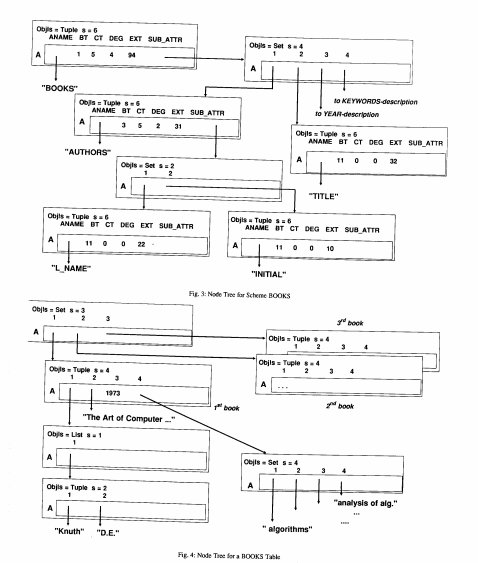
\includegraphics[scale=0.6]{Figures/VPDBEDIT.png}}
		\end{figure}

	\section{Libraries for Functionality}
		From GitHub Repositories, a list of Visual Scripting libraries are listed:-
		\begin{itemize}
		\item Language: GDScript - Author:~\href{https://github.com/swarnimarun}{Swarnimarun} - Respository:~\href{https://github.com/swarnimarun/visual-scripting-node-library}{Visual Scripting Node Library}.
		\item Language: Python - Author:~\href{https://github.com/leon-thomm}{leon-thomm} - Respository:~\href{https://github.com/leon-thomm/Ryven}{Ryven}.
		\item Language: C\# - Unity Game Engine - Author~\href{https://github.com/ConstellationLanguage}{ConstellationLanguage} - Respository:~\href{https://github.com/ConstellationLanguage/Constellation}{Constellation}.
		\item Language: Web Scripting - Author:~\href{https://github.com/ericabouaf}{ericabouaf} - Respository:~\href{https://github.com/ericabouaf/webhookit}{webhookit}.
		\item Language: Web Scripting - Author:~\href{https://github.com/WebCabin}{WebCabin} - Respository:~\href{https://github.com/WebCabin/wcPlay}{wcPlay}.
		\end{itemize}

		These Visual Scripting software listed are identical to standard Game Engine Visual Scripting logic. Even though some are easy to use in the demos, a commonality is that they only allow users to control a live environment, whether it is a built-in game engine or an addition to an existing Game Engine, and they are mainly game orientated. VisualPro aims to support different platforms, such as Web, Mobile, Software, Data Analytics and Games. This aim is possible due to the diversity of users, adding new languages by entering the desired language within the XML document; though, it requires documentation to support users in adding new languages for the program to work correctly.

		A table of a few Web Builders and Visual Scripters demonstrates the difficulty of different platforms. Visual Scripting Software~\ref{tab:comp-1}:-
		\begin{table}[htbp]
			\caption{Comparison of Visual Scripters}
			\label{tab:comp-1}
			
			\resizebox{\columnwidth}{!}{%
			\begin{tabular}{cccc}
			\hline
			\textbf{Name}                               & \textbf{Description}                                                                                     & \textbf{Difficulty: Hard (0-10) Easy}                   & \textbf{Explanation?}                                                                                                                                                                                                                      \\ \hline
			\multicolumn{1}{c|}{Unreal Engine 5~\cite{unreal_engine_introduction_nodate}} & \multicolumn{1}{c|}{Game Engine (C++ Language)}                                                          & \multicolumn{1}{c|}{Beginner: 3-0 | Experience: 5-10}   & \begin{tabular}[c]{@{}c@{}}A beginner who does not \\ understand the principles of code \\ may struggle over time.\end{tabular}                                                                                                            \\ \hline
			\multicolumn{1}{c|}{Unity Engine~\cite{unity_technologies_unity_nodate}}    & \multicolumn{1}{c|}{Game Engine (C\# Language)}                                                          & \multicolumn{1}{c|}{Beginner: 2 - 6 | Experience: 8-10} & \begin{tabular}[c]{@{}c@{}}With the documentation available\\ and the simplicity of the Unity\\ Visual Scripting design, it seems\\ beginner-friendly.\end{tabular}                                                                        \\ \hline
			\multicolumn{1}{c|}{Minecraft~\cite{mojang_minecraft_nodate}}       & \multicolumn{1}{c|}{\begin{tabular}[c]{@{}c@{}}Game (Redstone)\\ Represents binary coding.\end{tabular}} & \multicolumn{1}{c|}{Beginner: 7-10 | Experience: 10}    & \begin{tabular}[c]{@{}c@{}}Even though Minecraft does not\\ create programming languages,\\ it shows that many ages who enjoy\\ logging onto Minecraft to make\\ Redstone functionality, passively\\ learn about Binary code.\end{tabular} \\ \hline
			\end{tabular}%
			}
			\end{table}

			After studying different Visual Scripting software, there is no portable Visual Scripting made for versatility. Both seem to only aim at Game Engines. Minecraft does not offer the ability for Visual Scripting. However, to bring attention to the Redstone feature in Minecraft, the feature is interesting for the audience, even to none-programmers. Could the VisualPro library be made into a Visual Scripting game, or specific in-game blueprints/prefabs be placed into the environment, generating code, so that the user can create programs whilst maintaining interest? Redstone accomplishes Binary teaching with Redstone passively by using on and off instead of 1s and 0s.

			Visual Scripting, Unreal Engine has a `messy' look, especially when the game logic is more clunky and complex, whereas Unity seems to have a better order. The problem with Visual Scripting in both engines is that the performance of the code is slow compared to writing the code manually. Would this uplift the software market sections if the VisualPro Scripting Pad software could generate code in the desired language with the most effective running time?

			\begin{table}[htbp]
			\centering
			\caption{Comparison of Web Builders}
			\label{tab:comp-2}
			\resizebox{\columnwidth}{!}{%
			\begin{tabular}{cccc}
			\hline
			\textbf{Name}                                                                   & \textbf{Description}             & \textbf{Difficulty: Hard (0-10) Easy}                  & \textbf{Explanation?}                                                                                                                                                                                                                  \\ \hline
			\multicolumn{1}{c|}{WordPress}                                                  & \multicolumn{1}{c|}{Web Builder} & \multicolumn{1}{c|}{Beginner: 8-10 | Experience: 9-10} & \begin{tabular}[c]{@{}c@{}}WordPress offers many\\ themes and plugins\\ to the user base.\end{tabular}                                                                                                                                 \\ \hline
			\multicolumn{1}{c|}{Wix}                                                        & \multicolumn{1}{c|}{Web Builder} & \multicolumn{1}{c|}{Beginner: 9-10 | Experience: 10}   & \begin{tabular}[c]{@{}c@{}}Wix is designed to help\\ buisnesses to design\\ webpages with no skill\\ required.\end{tabular}                                                                                                            \\ \hline
			\multicolumn{1}{c|}{\begin{tabular}[c]{@{}c@{}}Bootstrap\\ Studio\end{tabular}} & \multicolumn{1}{c|}{Web Builder} & \multicolumn{1}{c|}{Beginner: 5-7 | Experience: 7-10}  & \begin{tabular}[c]{@{}c@{}}Bootstrap Studio is a\\ similar interface to\\ Adobe Dreamweaver.\\ It offers templates and\\ allowed websites to designed.\\ This interface is difficult with\\ no experience with Bootstrap.\end{tabular} \\ \hline
			\end{tabular}%
			}
			\end{table}

			In one form, Web Builder's give an idea of what makes Visual Scripting easier. This concept is down to the research, design, and implementation of existing developers who had to look into individuals with no coding experience. If there is a correlation between designing a more straightforward Visual Scripting interface using methods that Web Builders introduced, it could update Visual Scripting and bring it into future software design. Perhaps, it could be a tool to visualise JavaScript so that users can build a website and add functionality, or create code snippets, for example, MelPy to animate 3D models within Autodesk Maya and other products, making Artists thrive more rather than relying on a Software Engineer to make their vision.
	\section{Testing Funcionality}
	
\chapter{Research Methodology}
\label{chap:researchMethodology}

\chapter{Design and Feedback}
\label{chap:designAndFeedback}
	The Design and Feedback section covers the Research Methodology and the Pre-Planning, which shows the steps and the level of thought that went into deciding VisualPro's purpose and the existing software and prototypes. Some Notebook Planning may not make sense as some foreseeable problems were thought and planned ahead of time.
	
	\section{Pre-Planning}
		\subsection{HTML Design} 
			Figure~\ref{fig:htmlDesign} shows a HyperText Markup Language (HTML) Design of how the UI should look. The Empty Column is where the user drops elements like Classes, Functions or Variables. Buttons on the right can be dragged and dropped on the Empty Column to the left. The functionality of the drop should create a new container, giving the user acknowledgement there's a new parent or sub-element with room for configuration and another drag and drop container within the class or function.

			\begin{figure}[H]
				\ffigbox[\FBwidth] {
				\caption[UI Illustration]{HTML Design - Found at: \href{https://github.com/ShinkuKira21/VisualPro-FinalProject/blob/main/Showcase-Work_Completed/PrePlanning\%20(Whole\%20Idea)/HTML_Design.jpg}{Original Image}}
				\label{fig:htmlDesign}
				}
				{\includegraphics[scale=0.55]{{"../../Showcase-Work_Completed/PrePlanning (Whole Idea)/HTML_Design"}.jpg}}
			\end{figure}

		\subsection{Notebook Page 1-2} 
			Figure~\ref{fig:nb-1} contains numerous ideas. Page 1 contains a heading, 'Personal Assistant', which indicates the thought process of a personal assistant before the Visual Programming Scripting program progressed. After planning this, it became apparent to use a type of Artificial Intelligence (AI), which knew the basic syntax of different languages and would write or advise the user when typing. This process is very similar to TabNine~\cite{tabnine_code_nodate}.

			The second page of this figure, shows a few different examples of IF statement syntax from languages to find a `dynamic' common rather than keep it static like the previous software. The sketch below shows a name for the software and a example of how the language selection would look on UI.

			\begin{figure}[H]
				\ffigbox[\FBwidth] {
				\caption[Notebook P-1.2]{Notebook Plan Page 1-2 - Found at: \href{https://github.com/ShinkuKira21/VisualPro-FinalProject/blob/main/Showcase-Work_Completed/PrePlanning\%20(Whole\%20Idea)/NP1.jpg}{Original Image}}
				\label{fig:nb-1}
				}
				{\includegraphics[scale=0.45]{{"../../Showcase-Work_Completed/PrePlanning (Whole Idea)/NP1"}.jpg}}
			\end{figure}
			
		\subsection{Notebook Page 2-3} 
			Figure~\ref{fig:nb-2} displays two pages of how the Visual Scripting could look. The top page shows the tools on the left, such as Logical, Structure and Scoping tools. On the right, it should show a list of current variables, functions and classes in a hierarchy style. The middle of the application is the work area.
			\begin{figure}[H]
				\ffigbox[\FBwidth] {
				\caption[Notebook P-3.4]{Notebook Plan Page 3-4 - Found at: \href{https://github.com/ShinkuKira21/VisualPro-FinalProject/blob/main/Showcase-Work_Completed/PrePlanning\%20(Whole\%20Idea)/NP2.jpg}{Original Image}}
				\label{fig:nb-2}
				}
				{\includegraphics[scale=0.6]{{"../../Showcase-Work_Completed/PrePlanning (Whole Idea)/NP2"}.jpg}}
			\end{figure}

		\subsection{Notebook Page 5-6} 
			Figure~\ref{fig:nb-3} gives the planning of how the syntax for most programming and scripting languages. The plan points out patterns and tries to identify their names for the Extensible Markup Language (XML) and backend to comprehend. This piece of planning helped excel the development of the program's dynamic side to allow the addition of new languages to the software.
			\begin{figure}[H]
				\ffigbox[\FBwidth] {
				\caption[Notebook P-5.6]{Notebook Plan Page 5-6 - Found at: \href{https://github.com/ShinkuKira21/VisualPro-FinalProject/blob/main/Showcase-Work_Completed/PrePlanning\%20(Whole\%20Idea)/NP3.jpg}{Original Image}}
				\label{fig:nb-3}
				}
				{\includegraphics[scale=0.45]{{"../../Showcase-Work_Completed/PrePlanning (Whole Idea)/NP3"}.jpg}}
			\end{figure}

		\subsection{Notebook Page 7-8} 
			Figure~\ref{fig:nb-4} demonstrates how the XML would possibly look. The table shows N (Node), A (Attribute) and the Meaning. To explain what is going on, Node |0| is the header node (holds library data such as \textbf{system} or \textbf{iostream}), holds three attributes. Attribute |0| holds `Type', which is the purpose, Attribute |1| holds the `Name', which is the library's name. Attribute |2| holds the `Syntax Value', which in C\# it is \textit{using ;} and in C++, the value is \textit{\#include $<>$} .
	
			According to the second node |1| holds information for structure or classes in languages. This node contains three attributes. Attribute |0| holds `Name of Struct \textit{(or)} Class', which contains the user-defined name they have created inside VisualPro. Attribute |2| holds the `Properties' like the member of the struct/class. Attribute |3| holds the syntax value, the open and close case of a struct/class and layout within the struct/class.
	
			\begin{figure}[H]
				\ffigbox[\FBwidth] {
				\caption[Notebook P-7.8]{Notebook Plan Page 7-8 - Found at: \href{https://github.com/ShinkuKira21/VisualPro-FinalProject/blob/main/Showcase-Work_Completed/PrePlanning\%20(Whole\%20Idea)/NP4.jpg}{Original Image}}
				\label{fig:nb-4}
				}
				{\includegraphics[scale=0.45]{{"../../Showcase-Work_Completed/PrePlanning (Whole Idea)/NP4"}.jpg}}
			\end{figure}
	
		\subsection{Notebook Page 9-10}
			Figure~\ref{fig:nb-5} answers how the loops and logical statements work in the LanguageCompiler library. This planning shows how the XML nodes and the Planner List should work together. In theory, the Planner List, of what the user populates with the program's use, combines with the XML document with the chosen language.

			\begin{figure}[H]
				\ffigbox[\FBwidth] {
				\caption[Notebook P-9.10]{Notebook Plan Page 9-10 - Found at: \href{https://github.com/ShinkuKira21/VisualPro-FinalProject/blob/main/Showcase-Work_Completed/PrePlanning\%20(Whole\%20Idea)/NP5.jpg}{Original Image}}
				\label{fig:nb-5}
				}
				{\includegraphics[scale=0.45]{{"../../Showcase-Work_Completed/PrePlanning (Whole Idea)/NP5"}.jpg}}
			\end{figure}
	
		\subsection{Notebook Page 11} 
			Figure~\ref{fig:nb-6} displays how the function node should work. This miniature theory is to help the developer understand how the XML document should work in a programmatical sense. This again helped when it comes to the prototypes further in this document.
	
			\begin{figure}[H]
				\ffigbox[\FBwidth] {
				\caption[Notebook P-11]{Notebook Plan Page 11 - Found at: \href{https://github.com/ShinkuKira21/VisualPro-FinalProject/blob/main/Showcase-Work_Completed/PrePlanning\%20(Whole\%20Idea)/NP6.jpg}{Original Image}}
				\label{fig:nb-6}
				}
				{\includegraphics[scale=1]{{"../../Showcase-Work_Completed/PrePlanning (Whole Idea)/NP6"}.jpg}}
			\end{figure}
	
		%recheck-$41%
		\newpage
		\subsection{Notebook Page 12-13} 
			Figure~\ref{fig:nb-7} shows a predicted problem is as follows:
			\begin{center}
				\textbf{Description:}\\ How will the program know where to put a sub-child and how will it?
			
				\textbf{Answer:}\\ The planner would hold its parent and sub identity, and the Triangle (30 Code) symbol tells the software where to put the child. The Triangle symbol will only appear of classes or functions that have children. This means that the program will focus on parents, close the tags, then rescan to put the children in the code. The problem before is that it would be hard to tell the program to remember when and where to close tags if it got too deep in theory.
			\end{center}
	
			\begin{figure}[H]
				\ffigbox[\FBwidth] {
				\caption[Notebook P-12.13]{Notebook Plan Page 12-13 - Found at: \href{https://github.com/ShinkuKira21/VisualPro-FinalProject/blob/main/Showcase-Work_Completed/PrePlanning\%20(Whole\%20Idea)/NP7.jpg}{Original Image}}
				\label{fig:nb-7}
				}
				{\includegraphics[scale=0.45]{{"../../Showcase-Work_Completed/PrePlanning (Whole Idea)/NP7"}.jpg}}
			\end{figure}
	
		%recheck-$41%
		\newpage
		\section{Results of Feedback}
			\subsection{Survey Question 1} 
				According to the chart~\ref{fig:q-1}, \textit{87.5\%} chose `Programming Planner Improved', and \textit{12.5\%} chose `None of the Above' to the question, `As a developer, which program worked for you?'. This data suggests that most of the responses preferred `Programming Planner Improved' out of eight.
				\begin{figure}[H]
					\ffigbox[\FBwidth] {
					\caption[Survey Q-1]{Survey Question 1 - Found at: \href{https://github.com/ShinkuKira21/VisualPro-FinalProject/blob/main/Showcase-Work_Completed/Surveying/q1.png}{Original Image}}
					\label{fig:q-1}
					}
					{\includegraphics[scale=0.50]{{"../../Showcase-Work_Completed/Surveying/q1"}.png}}
				\end{figure}

			\subsection{Survey Question 2}
				Figure~\ref{fig:q-2} asks the question, `If the last option on the previous question is ticked, then explain why?'. Four responses replied with:-
				\begin{itemize}
					\item `More flexibility' -\\
							This response could mean two things: the Programming Planner Improved is more flexible than the first program or that both programs would benefit from more flexibility.
					\item `Both work' -\\
							This response indicates that both software works.
					\item `The option to choose the desired programming language at the end of the programming' -
							A surveyee liked the option in Programming Planner Improved to select different programming languages.
					\item `Because it had more options and had example code at the end of planning' -
							This answer describes that the Programming Planner Improved offered more options, such as argument selection and code language.
				\end{itemize}
		
				\begin{figure}[H]
					\ffigbox[\FBwidth] {
					\caption[Survey Q-2]{Survey Question 2 - Found at: \href{https://github.com/ShinkuKira21/VisualPro-FinalProject/blob/main/Showcase-Work_Completed/Surveying/q2.png}{Original Image}}
					\label{fig:q-2}
					}
					{\includegraphics[scale=0.45]{{"../../Showcase-Work_Completed/Surveying/q2"}.png}}
				\end{figure}
		
			\subsection{Survey Question 3} 
				Figure~\ref{fig:q-3} asks the question to Surveyee's, `Did the tutorial at the beginning of Programming Planner Improved help navigate around the application?'. This question tries to find out if the application is hard to use overall. The responses were 87.5\% for yes, and 12.5\% for no. Even though the most of the responses chose yes, the application may still be hard to use if, theoretically, one out of eight users found the User Experience frustrating or confusing.

				\begin{figure}[H]
					\ffigbox[\FBwidth] {
					\caption[Survey Q-3]{Survey Question 3 - Found at: \href{https://github.com/ShinkuKira21/VisualPro-FinalProject/blob/main/Showcase-Work_Completed/Surveying/q3.png}{Original Image}}
					\label{fig:q-3}
					}
					{\includegraphics[scale=0.45]{{"../../Showcase-Work_Completed/Surveying/q3"}.png}}
				\end{figure}
		
			\subsection{Survey Question 4}
				Figure~\ref{fig:q-4}, `What makes the Programming Planner Improved better than the previous product?' checkbox question, offered five qualities. These are:-
				\begin{itemize}
					\item \textbf{Ease of Use} - Aimed to find out how easy the application is easy to use. 50\% of the responses think it was easier to use than the previous product. This feedback could mean to things, the first product was similar and consequently did not improve the application in this quality or that the product needs to improve in this area.
					\item \textbf{Performance} - To see if the audience could notice any performance difference. This quality is vital as a Graphical User Interface (GUI) can somewhat be `chunky'. The responses were 0\% out of the responses; though this may seem negative, it is sometimes hard to notice the difference between console and desktop applications.
					\item \textbf{Extra Features} - The quality, `Extra Features`, displays if the extra features in the new application stood out and improved the previous application. The responses were 62.5\%, which indicates that the extra features did stand out and made the application better.
					\item \textbf{File Structure} - The quality, `File Structure' of the second application is revised and stores the saved file in a directory other than the ROOT directory. 25\% of the responses chose this option, which means that the File Structure did not impact the application as effectively as the `Extra Features' quality.
				\end{itemize}

				\begin{figure}[H]
					\ffigbox[\FBwidth] {
					\caption[Survey Q-4]{Survey Question 4 - Found at: \href{https://github.com/ShinkuKira21/VisualPro-FinalProject/blob/main/Showcase-Work_Completed/Surveying/q4.png}{Original Image}}
					\label{fig:q-4}
					}
					{\includegraphics[scale=0.45]{{"../../Showcase-Work_Completed/Surveying/q4"}.png}}
				\end{figure}
		
			\subsection{Survey Question 5}
				Figure~\ref{fig:q-5} asks the Surveyee's, `Explain your answer' to the last question. This question will tell what the Surveyee's felt when answering the last question. The responses are as follows:
				\begin{itemize}
					\item `More features allowed for a wider range of approaches' - This specific feedback suggests that it is better to add more functionality in the GUI application to allow for more usability.
					\item `More languages and was easier to use. Very impressed' - This response implies that the idea of a dynamic language interface to allow users to add more languages will increase User Experience.
					\item `Easier to use, the better' - Visual Scripting already is complicated when looking at the Unreal Engine's Visual Scripting interface. If it is possible to create a lightweight Visual Scripting pad to allow a programmer to create code snippets, it could bring more developers into the field and increase production time already in the field.
					\item `Have not used the previous version' - This suggests that the Surveyee only tested Programming Planner Improved.
					\item `Allowed me to create a function structure and save it. Seemed difficult to follow (variables weren' numbered)' - According to this response, the user found it difficult to follow through and should be something to think about when making the GUI application.
					\item `Easy, helpful and understandable' - This response shows that the user found the software easy to use, helpful and understanding during their experience.
					\item `The extra features added to the improved version of the program improve used experience by adding expanded usability' - The response suggests that again the extra functionality helped improve the User Experience, in Programmer Planner Improved.
					\item `It just had extra features and seemed more useful' - Which implies that the user found the extra features more comfortable and useful to use.
				\end{itemize}
		
				\begin{figure}[H]
					\ffigbox[\FBwidth] {
					\caption[Survey Q-5]{Survey Question 5 - Found at: \href{https://github.com/ShinkuKira21/VisualPro-FinalProject/blob/main/Showcase-Work_Completed/Surveying/q5.png}{Original Image}}
					\label{fig:q-5}
					}
					{\includegraphics[scale=0.45]{{"../../Showcase-Work_Completed/Surveying/q5"}.png}}
				\end{figure}
		
			\subsection{Survey Question 6}
				Figure~\ref{fig:q-6} asks the Surveyee, `How would you rate the User Experience (overall)?'. The question tries to aim for an idea of how the UX of the two products. On a scale of one (Stressful) to ten (Relaxing), 62.5\% of the responses went with option eight, 37.5\% of the responses went with option seven. These figures show that the UX has room for improvement. When designing and implementing the GUI product, it is important to think about the UI and UX.

				\begin{figure}[H]
					\ffigbox[\FBwidth] {
					\caption[Survey Q-6]{Survey Question 6 - Found at: \href{https://github.com/ShinkuKira21/VisualPro-FinalProject/blob/main/Showcase-Work_Completed/Surveying/q6.png}{Original Image}}
					\label{fig:q-6}
					}
					{\includegraphics[scale=0.45]{{"../../Showcase-Work_Completed/Surveying/q6"}.png}}
				\end{figure}
				
			\subsection{Survey Question 7}
				Figure~\ref{fig:q-7} asks the question, `How useful is Programming Planner for beginners?'. This question is done on a scale of one (Complicated) to five (Useful). The feedback is ranged from one to five and suggests that beginners may find this platform hard work. The responses are as follows:
				\begin{itemize}
					\item \textbf{One} - 25\% responses. These respondents reckon that Programming Planner is complicated for beginners.
					\item \textbf{Three} - 12.5\% responses. These respondents thought that Programming Planner is a little complicated for beginners.
					\item \textbf{Five} - 50\% responses. These respondents figure that Programming Planner is close to Useful for beginners.
					\item \textbf{Six} - 12.5\% responses. These respondents consider that Programming Planner is Useful for beginners. 
				\end{itemize}
		
				\begin{figure}[H]
					\ffigbox[\FBwidth] {
					\caption[Survey Q-7]{Survey Question 7 - Found at: \href{https://github.com/ShinkuKira21/VisualPro-FinalProject/blob/main/Showcase-Work_Completed/Surveying/q7.png}{Original Image}}
					\label{fig:q-7}
					}
					{\includegraphics[scale=0.45]{{"../../Showcase-Work_Completed/Surveying/q7"}.png}}
				\end{figure}
				
			\subsection{Survey Question 8}
				Question~\ref{fig:q-8} `Did this help create a structure of your favourite language faster than standard methods?'. 75\% of responses said Yes, 12.5\% of responses said `Would not recommend to new programmer as they will not learn the basics' and 12.5\% said `I have not used other methods'. This chart suggests that the majority found this software to be faster than their standard methods.
				\begin{figure}[h]
					\centering
					\includegraphics[width=0.85\columnwidth]{{"../../Showcase-Work_Completed/Surveying/q8"}.png}
					\caption{Survey Question 8 - Found at: \href{https://github.com/ShinkuKira21/VisualPro-FinalProject/blob/main/Showcase-Work_Completed/Surveying/q8.png}{Original Image}}
					\label{fig:q-8}
				\end{figure}
		
			\subsection{Survey Question 9}
				Question~\ref{fig:q-9} `What features would you wish Programming Planner to offer?'. This question attempts to determine if the user has any requests about the software they have used. These were the responses:-
				\begin{itemize}
					\item `When I wanted only one function on the variable creation it asked if it works with other functions but I didn't have any other functions' - This suggestion shows that the user was confused with the way the program asked the user if the variable was a argument or a standard variable.
					\item `The target audience for this program will have little coding experience, and may forget what is required of a function, variable, etc. Adding examples to each page may be a good idea to reduce confusing.' - This suggestion shows that a help page or tips pop up on creating an element within the GUI program will help beginners use this software.
					\item `A set of pre made open source programs that could be quickly accessed' - Perhaps, the program could offer a GitHub repository import, which will examine the code and visualise it for the user.
					\item `Would be better with visualisation if writing a longer program' - The response could mean two things. It could mean that the user wanted to have an ability to overview the code within the console application, or it could mean that the user would have preferred a GUI work area.
					\item `A GUI' - This response means that the user would have preferred a GUI product rather than a console application.
					\item `Allow sudo code comments to be added to the function' - In the GUI application, it could have the ability for the user to enter comments.
					\item `Calculator?' - This response did not seem useful to add in to the future software, as popup calculators are available in most operating systems.
				\end{itemize}
		
				\begin{figure}[H]
					\ffigbox[\FBwidth] {
					\caption[Survey Q-9]{Survey Question 9 - Found at: \href{https://github.com/ShinkuKira21/VisualPro-FinalProject/blob/main/Showcase-Work_Completed/Surveying/q9.png}{Original Image}}
					\label{fig:q-9}
					}
					{\includegraphics[scale=0.45]{{"../../Showcase-Work_Completed/Surveying/q9"}.png}}
				\end{figure}
		
			\subsection{Survey Question 10}
				Figure~\ref{fig:q-10} ask `Would a Graphical User Interface uplift the User Experience?' as a multiple-choice question. The 100\% chose the yes choice. This feedback implies that they would like a GUI to work with over a console application out of the eight responses.
				\begin{figure}[H]
					\ffigbox[\FBwidth] {
					\caption[Survey Q-11]{Survey Question 10 - Found at: \href{https://github.com/ShinkuKira21/VisualPro-FinalProject/blob/main/Showcase-Work_Completed/Surveying/q10.png}{Original Image}}
					\label{fig:q-10}
					}
					{\includegraphics[scale=0.45]{{"../../Showcase-Work_Completed/Surveying/q10"}.png}}
				\end{figure}
		
			\subsection{Survey Question 11} 
				A grid question asked `According to you, how should the features of the Graphical User Interface have to work?'. The following options are: `Clickable', `Drag and Drop', `Drop Down Menu' and `Text Filled'. The details are `Structure Elements', `Logic Elements', `Select Languages and Save' and `Sub Elements'. After overlooking the table~\ref{fig:q-11} `Structure Elements' looks like it favoured Drag and Drop the most by four responses. The Drag and Drop were also voted for the `Logic Elements' by five responses. The `Select Languages and Save' preferred the Drop Down Menu by six responses, and lastly, the `Sub Elements' liked the idea if it was Text Filled.

				\begin{figure}[H]
					\ffigbox[\FBwidth] {
					\caption[Survey Q-11]{Survey Question 11 - Found at: \href{https://github.com/ShinkuKira21/VisualPro-FinalProject/blob/main/Showcase-Work_Completed/Surveying/q11.png}{Original Image}}
					\label{fig:q-11}
					}
					{\includegraphics[scale=0.45]{{"../../Showcase-Work_Completed/Surveying/q11"}.png}}
				\end{figure}
		
			\subsection{Survey Question 12} 
				This grid asks the participants, `How would you prefer to access the software?'. The options are `Windows Operating System', `Linux Operating System', `ChromeOS/Android' and `iOS'. The details are `Computer, Laptop or Tablet Devices', `Web Application', `Mobile Devices'. For the first column, the responses favour the Windows Operating System by eight. The second column, Windows Operating System, is also preferred by eight. The last column, ChromeOS, is the six responses favourites, and iOS is preferred by four. After reviewing this, the application aims for the Windows Operating System to get the most attention. Programming Planner and Programming Planner Improved works for both Windows and Linux Operating Systems.
				\begin{figure}[H]
					\ffigbox[\FBwidth] {
					\caption[Survey Q-12]{Survey Question 12 - Found at: \href{https://github.com/ShinkuKira21/VisualPro-FinalProject/blob/main/Showcase-Work_Completed/Surveying/q12.png}{Original Image}}
					\label{fig:q-12}
					}
					{\includegraphics[scale=0.45]{{"../../Showcase-Work_Completed/Surveying/q12"}.png}}
				\end{figure}
		
			\subsection{Survey Question 13}
				Figure~\ref{fig:q-13} a question, `Any comment?' follows the last questions. The only response was `No'.

				\begin{figure}[H]
					\ffigbox[\FBwidth] {
					\caption[Survey Q-13]{Survey Question 13 - Found at: \href{https://github.com/ShinkuKira21/VisualPro-FinalProject/blob/main/Showcase-Work_Completed/Surveying/q13.png}{Original Image}}
					\label{fig:q-13}
					}
					{\includegraphics[scale=0.45]{{"../../Showcase-Work_Completed/Surveying/q13"}.png}}
				\end{figure}
		
			\subsection{Survey Question 14-15}
				Figures~\ref{fig:q-14} and~\ref{fig:q-15} shows two questions, `How complicated is Visual Scripting? (Reference to Unreal Engine for an example).' Furthermore, `How complicated is Website Builders?' these questions portray how existing Visual Scripting Web Builders are successful, and if it is possible to do a service that is easier to use, similar to a web builder. The question is on a scale of one (Piece of Cake) to five (Complicated). The feedback from the first question:-
				\begin{itemize}
					\item Three - 37.5\% of the responses. This indicates that this percentage of the participants find Visual Scripting moderately easy.
					\item Four - 50\% of the responses. This displays that 50\% of the participants find Visual Scripting a bit more complicated than the 37.5\%.
					\item Five - 12.5\% of the responses find Visual Scripting tough.
				\end{itemize}
		
				The feedback from the second question:-
				\begin{itemize}
					\item One - 25\% of the responses find Web Builders a `Piece of Cake'.
					\item Two - 50\% of the responses find Web Builders more or less easy.
					\item Three - 25\% of the responses find Web Builders moderately easy.
				\end{itemize}
		
				These findings will change the research perspective to look more into the Web Builder layouts, functionality and UX to work out the GUI of the product.
		
				\begin{figure}[H]
					\ffigbox[\FBwidth] {
					\caption[Survey Q-14]{Survey Question 14 - Found at: \href{https://github.com/ShinkuKira21/VisualPro-FinalProject/blob/main/Showcase-Work_Completed/Surveying/q14.png}{Original Image}}
					\label{fig:q-14}
					}
					{\includegraphics[scale=0.45]{{"../../Showcase-Work_Completed/Surveying/q14"}.png}}
				\end{figure}

				\begin{figure}[H]
					\ffigbox[\FBwidth] {
					\caption[Survey Q-15]{Survey Question 15 - Found at: \href{https://github.com/ShinkuKira21/VisualPro-FinalProject/blob/main/Showcase-Work_Completed/Surveying/q15.png}{Original Image}}
					\label{fig:q-15}
					}
					{\includegraphics[scale=0.45]{{"../../Showcase-Work_Completed/Surveying/q15"}.png}}
				\end{figure}
		
			\subsection{Survey Question 16}
				Question~\ref{fig:q-16}, `If Programming Planner had an easy-to-use drag and drop feature without input and output relationships, then will this improve Visual Scripting overall?', the question paints a picture from the participants to see if the relationships in Visual Scripting that is similar to Entity-Relationship Diagrams if they cause a problem. All eight responses replied back with yes.

				\begin{figure}[H]
					\ffigbox[\FBwidth] {
					\caption[Survey Q-16]{Survey Question 16 - Found at: \href{https://github.com/ShinkuKira21/VisualPro-FinalProject/blob/main/Showcase-Work_Completed/Surveying/q16.png}{Original Image}}
					\label{fig:q-16}
					}
					{\includegraphics[scale=0.45]{{"../../Showcase-Work_Completed/Surveying/q16"}.png}}
				\end{figure}
		
			\subsection{Survey Question 17}
				Similar to the previous question to paint an image from what the participants want to see, `Would Visual Scripting be better if it allowed users to add any language they wish and generate any language with one click of a button?'. According to the figure~\ref{fig:q-17}, all of the eight responses responded with yes.

				\begin{figure}[H]
					\ffigbox[\FBwidth] {
					\caption[Survey Q-17]{Survey Question 17 - Found at: \href{https://github.com/ShinkuKira21/VisualPro-FinalProject/blob/main/Showcase-Work_Completed/Surveying/q17.png}{Original Image}}
					\label{fig:q-17}
					}
					{\includegraphics[scale=0.45]{{"../../Showcase-Work_Completed/Surveying/q17"}.png}}
				\end{figure}
		
			\subsection{Survey Question 18} 
				To squeeze more information from the participants, a question, `What was the reason for your selection?' was asked and made compulsory. The responses are as follows:-
				\begin{itemize}
					\item `Would be easier to write programs (for some people)'
					\item `A feature such as this would greatly reduce the production times involved in program development.'
					\item `save time and allow users to focus on the details'
					\item `I would like to code in any language I choose if that option was applicable.'
					\item `Useful feature'
					\item `Makes it more visual'
					\item `Again, the easier to use, and the more features, the better'
					\item `More accessibility'
				\end{itemize}
		
				After reading the feedback, a few points are to address. The current software already makes it easier to write code for some people, so it is imperative that the new software does not distract but improve the capability of writing software. The command-line may benefit users as it keeps developers in a similar environment they are probably already using. Another point to address is this question, `Will the GUI software get too heavy with too many features making it no longer lightweight?'. The best thing about having Dynamic-Link Libraries is that developers can incorporate into Java Android, iOS, Web Applications and, but not limited to, Visual Studio Code Extensions. The backend can open a `can of worms' to allow different interfaces to the top of the backend, like digital notebooks or other ideas. Anyone who develops on top of the backend can make any interfaces or even new scripting languages. This idea, in turn, will enable others to make it easier to use Visual Scripting and Languages to Write. For example, Python or JavaScript has the potential of being converted into C++ and vice-versa.

				\begin{figure}[H]
					\ffigbox[\FBwidth] {
					\caption[Survey Q-18]{Survey Question 18 - Found at: \href{https://github.com/ShinkuKira21/VisualPro-FinalProject/blob/main/Showcase-Work_Completed/Surveying/q18.png}{Original Image}}
					\label{fig:q-18}
					}
					{\includegraphics[scale=0.45]{{"../../Showcase-Work_Completed/Surveying/q18"}.png}}
				\end{figure}
		
			\subsection{Survey Question 19}
				Final question which asked the participant, `Would you like to leave any extra feedback?', which hopefully gets any extra feedback that the survey missed out. Six responses, excluding two including the response `No', are displayed below:-
				\begin{itemize}
					\item `Introducing both drag and drop, as well as text filled features will appeal to both beginners and experienced programmers.' - The reply suggests that both Drag and Drop menus and Text Filled features will appeal to both programmers than just one of the methods used. Another idea this program opens up is creating snippets that can work in Visual Studio Extension, giving the user more flexible tools for development.
					\item `A training manaul along with some begginer tutorials would really help new users get to grips with the software' - A training manual or documentation would benefit both the console and GUI applications.
					\item `Command-line is hard on eyes when using. Not very good for Visual Scripting in general.' - The best thing about the console application is that it already has a language compiler, which plays a massive part to give the GUI application a backend. However, this response backs up the reasoning why the frontend matters in this project.
					\item `Nothing besides a nice GUI' - Many Visual Scripting is done in GUI applications, so it was unusual for a console application to have achieved a similar result. 
				\end{itemize}
		
				\begin{figure}[H]
					\ffigbox[\FBwidth] {
					\caption[Survey Q-19]{Survey Question 19 - Found at: \href{https://github.com/ShinkuKira21/VisualPro-FinalProject/blob/main/Showcase-Work_Completed/Surveying/q19.png}{Original Image}}
					\label{fig:q-19}
					}
					{\includegraphics[scale=0.45]{{"../../Showcase-Work_Completed/Surveying/q19"}.png}}
				\end{figure}
			
		\section{Evaluation of Feedback}
			
		\section{Designs}
			\subsection{Main Layout}
				\begin{figure}[H]
					\ffigbox[\FBwidth] {
					\caption[GUI Design ML-1]{Design Planning - Stage 1}
					\label{fig:guiDesignML-1}
					}
					{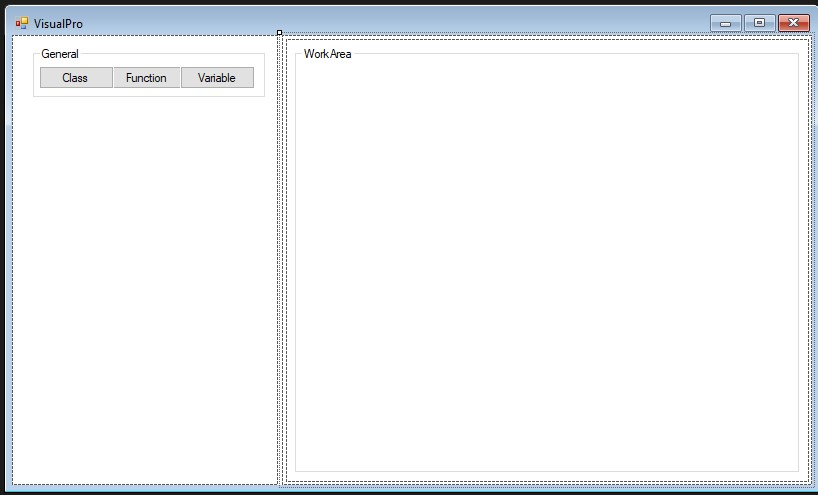
\includegraphics[scale=0.45]{Figures/vp-designs/NET_Framework-GUI-1.jpg}}
				\end{figure}

				\begin{figure}[H]
					\ffigbox[\FBwidth] {
					\caption[GUI Design ML-2]{Design Planning - Stage 2}
					\label{fig:guiDesignML-2}
					}
					{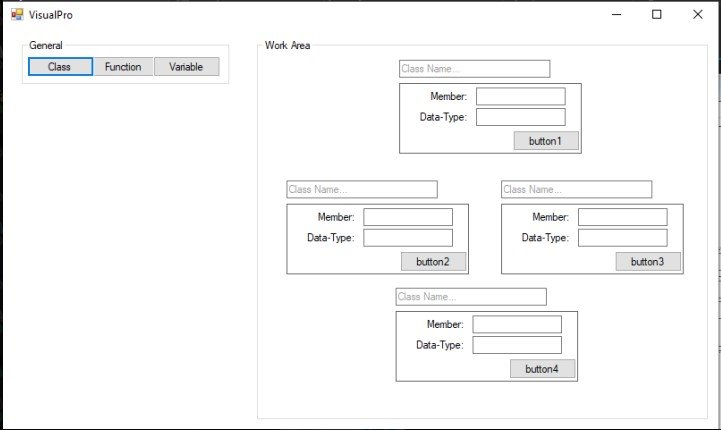
\includegraphics[scale=0.45]{Figures/vp-designs/NET_Framework-GUI-2-1.jpg}}
				\end{figure}

				A flaw of Classes', Functions and Variables' can be declared during development under the parent class. This problem meant that the class would be declared inside another class programmatically if the problem occurred under the current logic when the compilation happened. An example could be an \textit{`int variable = int variable;'}. The code syntax makes no sense, resulting in a compilation error.
				\begin{figure}[H]
					\ffigbox[\FBwidth] {
					\caption[GUI Design ML-3]{Design Planning - Stage 3}
					\label{fig:guiDesignML-3}
					}
					{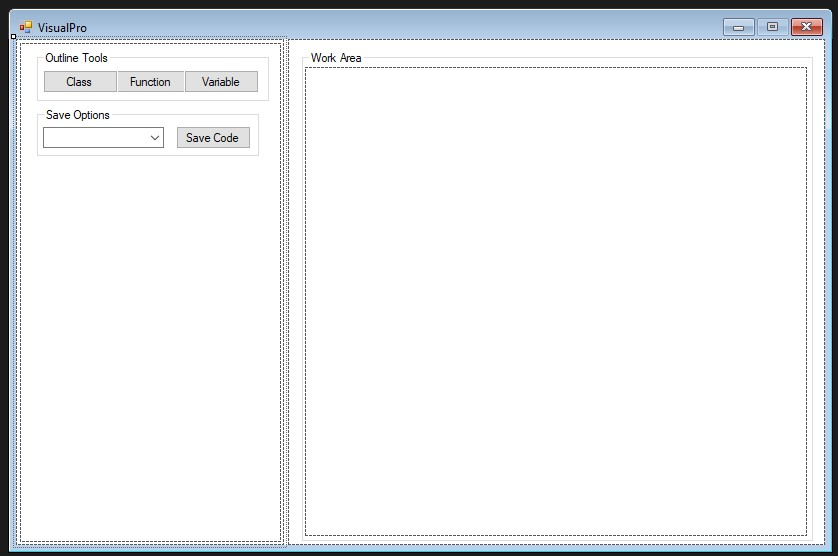
\includegraphics[scale=0.45]{Figures/vp-designs/NET_Framework-GUI-4.jpg}}
				\end{figure}

				Figure~\ref{fig:guiDesignML-4} shows the implementation of the design using the designs shown beforehand. Rather than shortcutting relationships between each class, function and variables by nesting them, the final implementation prevents the user from dragging and dropping the same type of container onto another container. A property button appears on each container to control function arguments and relationships between classes, functions, and variables, opening up a dialogue containing a property sheet.
				\begin{figure}[H]
					\ffigbox[\FBwidth] {
					\caption[GUI Design ML-4]{Design Planning - Stage 4}
					\label{fig:guiDesignML-4}
					}
					{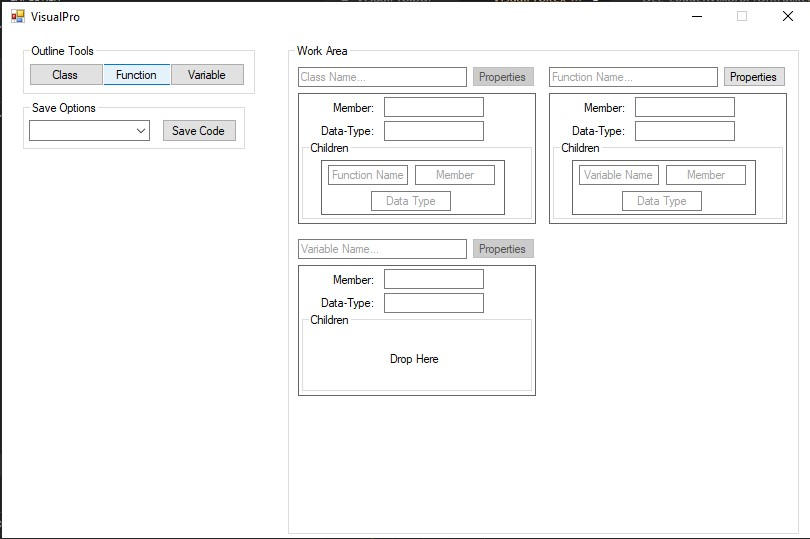
\includegraphics[scale=0.45]{Figures/vp-designs/NET_Framework-GUI-Latest.jpg}}
				\end{figure}
			
			\subsection{Error Handling}
				\begin{figure}[H]
					\ffigbox[\FBwidth] {
					\caption[GUI Design EH-1]{Error Handling}
					\label{fig:guiDesignEH-1}
					}
					{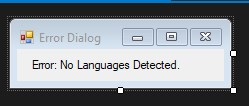
\includegraphics[scale=0.75]{Figures/vp-designs/NET_Framework-GUI-ErrorDialog.jpg}}
				\end{figure}
			\subsection{Structure Containers}
				\begin{figure}[H]
					\ffigbox[\FBwidth] {
					\caption[GUI Design SC-1]{Design Planning - Stage 1}
					\label{fig:guiDesignSC-1}
					}
					{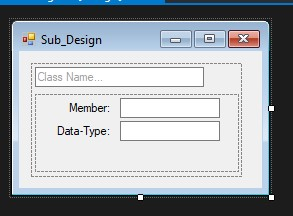
\includegraphics[scale=0.75]{Figures/vp-designs/NET_Framework-GUI-2.jpg}}
				\end{figure}
	\chapter{Development Methodology}

	\chapter{Implementation}
	
	\chapter{Evaluation}

	\chapter{Conclusion}

	\chapter{Reflection}

	\chapter{Terminology}
		List of terminologies used in this document:-
		\begin{itemize}
		\item UI - User Interface.
		\item UX - User Experience.
		\item UML - Unified Modeling Languages.
		\item OOP - Object-Orientated Programming.
		\item FP - Functional Programming.
		\item DLL - Dynamic-link Library.
		\item HTML - HyperText Markup Language.
		\item AI - Artificial Intelligence.
		\item XML - Extensible Markup Language.
		\item GUI - Graphical User Interface.
		\end{itemize}

	\chapter*{Acknowledgement}
		%Many thanks to the Supervisor, Mike Dacey, for guiding the VisualPro project with possibilities and for pointing out any discrepancies through the research, planning and implementation.
		Appreciation goes out to the survey participants, which helped better understand how VisualPro may impact consumers in the future. Having the support from these participants helped advance the UI and UX progress of VisualPro.
%----------
%	Bibliography
%----------	

\clearpage
\nocite{*}
\small{\bibliographystyle{IEEEtran}
\bibliography{ref}}

%----------
%	Appendix
%----------	

% If your work includes Appendix, you can uncomment the following lines
%\chapter* {Appendix x}
%\pagenumbering{gobble} % Appendix pages are not numbered

\end{document}